%!TEX root = main.tex
\setcounter{chapter}{3}
\setcounter{section}{2}
\setcounter{theorem}{0}
\setcounter{equation}{0}

\lectureheader{161}{Calculus I}{Derivatives}{\textit{Thomas' Calculus} \thesection}

\begin{definition}[Differentiability at a point]
Let $f$ be a function, and let $x_0\in\dom(f)$.
The \textbf{derivative of $f$ at $x_0$} is
\begin{equation*}
\left.\frac{\dee f}{\dee x}\right|_{x=x_0}=f'(x_0) = \lim_{h\to 0}\frac{f(x_0+h) - f(x_0)}{h}
\end{equation*}
provided that the limit exists.
When the limit exists, we say that $f$ is \textbf{differentiable at $x=x_0$.}
\end{definition}

\begin{center}
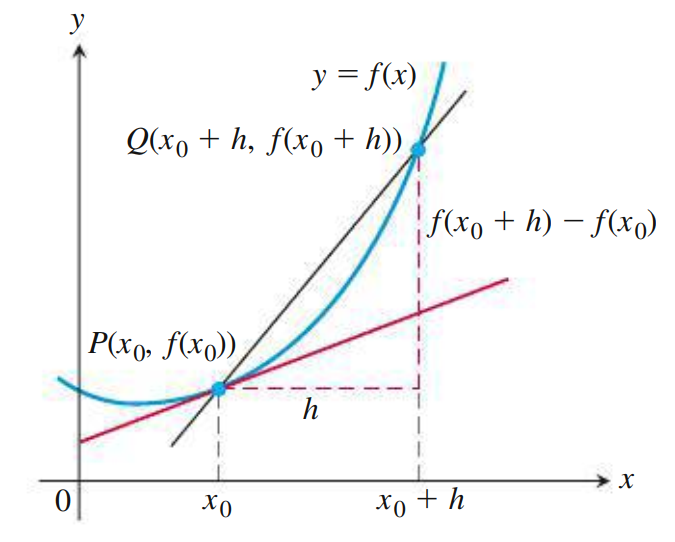
\includegraphics[width=3in]{img/derivative_as_slope}
\end{center}

\begin{remark}\,
\begin{enumerate}
\item If $f'(x_0)$ exists, then
\begin{itemize}
\item it is the slope of the tangent line to the curve $y=f(x)$ at $x=x_0$.
\item it is the (instantaneous) rate of change of $f$ with respect to $x$ at $x=x_0$.
\end{itemize}
\item If $\DS\lim_{h\to 0}\frac{f(x_0+h) - f(x_0)}{h}=\pm\infty$, then we say that the graph of $y=f(x)$ has a vertical tangent line at $x=x_0$.
(Note: In this case, we still say that the derivative does not exist.)
\end{enumerate}
\end{remark}

\newpage

\begin{example}
Let $y=\frac{1}{x}$.
\begin{enumerate}
\item What is the slope of the curve at $x=a\ne 0$?
\vfill
\item Where is the slope equal to $-1/4$?
\vfill
\end{enumerate}
\end{example}

\newpage

\begin{example}
Does the graph of 
\begin{equation*}
f(x) = \begin{cases}
x^2\sin(1/x) & \text{if }x\ne 0,\\
0 & \text{if }x=0
\end{cases}
\end{equation*}
have a tangent line at $x=0$?
What about 
\begin{equation*}
g(x) = \begin{cases}
x\sin(1/x) & \text{if }x\ne 0,\\
0 & \text{if }x=0?
\end{cases}
\end{equation*}
\end{example}
\begin{center}
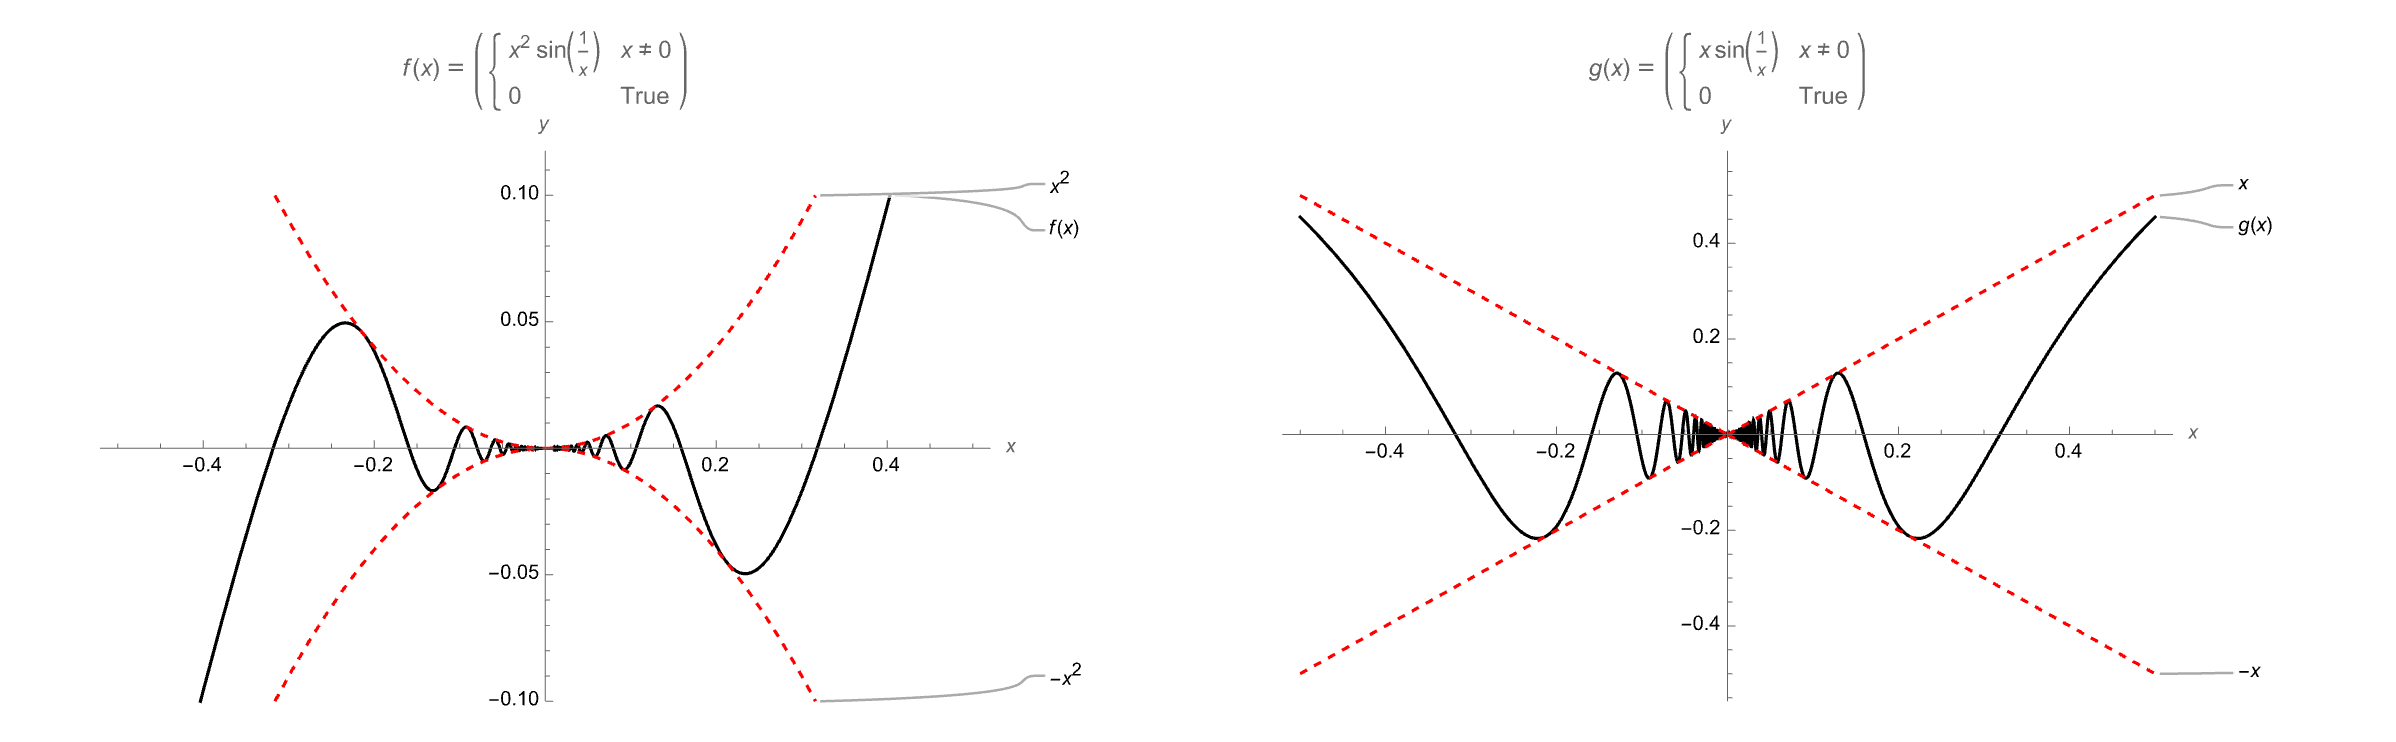
\includegraphics[width=6.5in]{img/osc_ex}
\end{center}

\newpage

\begin{example}
Show that the graph of $y=\sqrt[3]{x}$ has a vertical tangent at $x=0$.
\end{example}

\newpage

\begin{definition}[One-sided derivatives]
Let $f$ be a function, and let $x_0\in\dom(f)$.
The \textbf{right-hand derivative of $f$ at $x=x_0$} is
\begin{equation*}
D_+f(x_0) = \lim_{h\to 0^+}\frac{f(x_0+h)-f(x_0)}{h}
\end{equation*}
provided that the limit exists, in which case we say that $f$ is \textbf{right-differentiable at $x=x_0$}.
The \textbf{left-hand derivative of $f$ at $x=x_0$} is
\begin{equation*}
D_-f(x_0) = \lim_{h\to 0^-}\frac{f(x_0+h)-f(x_0)}{h}
\end{equation*}
provided that the limit exists, in which case we say that $f$ is \textbf{left-differentiable at $x=x_0$}.
\end{definition}

\begin{theorem}
Suppose that $f$ is defined on an open interval containing $c$.
Then $f'(c)=m$ if and only if $D_+f(c)=m=D_-f(c)$.
\end{theorem}

\begin{definition}[Differentiability on an interval]\,
\begin{itemize}
\item We say that $f$ is \textbf{differentiable on the open interval $(a,b)$} if it is differentiable at every point $c\in (a,b)$.
\item We say that $f$ is \textbf{differentiable on the closed interval $[a,b]$} if
\begin{enumerate}
\item it is differentiable at every point $c\in (a,b)$,
\item it is right-differentiable at $a$, and
\item it is left-differentiable at $b$.
\end{enumerate}
\end{itemize}
\end{definition}

%\begin{remark}\,
%\begin{itemize}
%\item The graph of $y=f(x)$ will have a \textbf{corner} at $x=c$ if
%\begin{enumerate}
%\item $D_+f(c)$ and $D_-f(c)$ both exist, but
%\item $D_+f(c)\ne D_-f(c)$.
%\end{enumerate}
%\item The graph of $y=f(x)$ will have a \textbf{vertical tangent} at $x=c$ if
%\begin{equation*}
%\DS\lim_{h\to 0}\frac{f(c+h) - f(c)}{h}=\pm\infty.
%\end{equation*}
%
%\end{itemize}
%no corners, cusps, vertical tangents, or ``wild" oscillations
%\end{remark}



\newpage

\begin{definition}
Let $f$ be a function of $x$.
The \textbf{derivative of $f$ with respect to $x$} is the function $f'$ given by the rule
\begin{equation*}
f'(x) = \lim_{h\to 0}\frac{f(x+h) - f(x)}{h}
\end{equation*}
and whose domain is the set of $x$ for which the limit exists.
\end{definition}
\begin{remark}
It is also common to denote the derivative by $\frac{\dee f}{\dee x}$.
\begin{itemize}
\item This more explicit notation due to Leibniz helps remind us that the derivative means the (instantaneous) rate of change in $f$ with respect to $x$.
\item In application, the units of $\frac{\dee f}{\dee x}$ are $f$-units per $x$-unit.
\end{itemize}
\end{remark}

\begin{example}
Differentiate $\DS f(x) = \frac{x}{x-1}$ with respect to $x$.
\end{example}

\newpage

\begin{example}\,
\begin{enumerate}
\item Compute the derivative of $f(x)=\sqrt x$ and its domain.
\vfill
\item Determine the tangent line to $y=\sqrt x$ at $x=4$.
\vfill
\end{enumerate}
\end{example}

\newpage

\begin{example}
Determine where $y=|x|$ is differentiable.
\end{example}

\newpage

\begin{theorem}
If $f$ is differentiable at $x=c$, then $f$ is continuous at $x=c$.
\end{theorem}
\begin{remark}\,
\begin{itemize}
\item The above theorem tells us that if $f$ is not continuous at $x=c$, then $f$ cannot be differentiable at $x=c$.
\item However, $f$ can be continuous without being differentiable.
\item The graph of a differentiable function is \textit{smooth}: no corners, cusps, vertical tangents, or ``wild" oscillations.
\end{itemize}
\end{remark}

\newpage

\begin{example}
Water is being drained from a cylindrical tank over the course of an hour.
The volume of water in the tank after $t$ minutes is 
\begin{equation*}
V(t) = 10^5\left(1-\frac{1}{60}t\right)^2
\end{equation*}
gallons.  
Compute and interpret the derivatives $\left.\frac{\dee V}{\dee t}\right|_{t=10}$ and $\left.\frac{\dee V}{\dee t}\right|_{t=20}$.
\end{example}

